If you haven't downloaded and unzipped \href{https://libaoj.in/courses/2021f/MATH3341/zip/Math.3341.zip}{\texttt{Math.3341.zip}}. Download and unzip it under \verb|H:| (H Drive if you are working on the Remote Lab). Change the current working directory by typing \verb|cd H:\Math.3341\Math.3341.Lab.04| in the Command Window, and type \verb|edit lab_04_script| in the Command Window to edit \verb|lab_04_script.m|.

%---------------------------------------------
\section{Basics of Plotting Functions}
%---------------------------------------------
\begin{enumerate}[(a)]
    \item \label{enu:1a} Plot $y = x^3$. Define a vector \verb|x|, of which the range is from $-10$ to $10$ with step size $4$, then define \verb|y| by aforementioned $y$. Plot in \verb|subplot(2, 2, 1)|. Add labels \verb|$x$|, \verb|$y$| to $x$, $y$ axis, respectively, and add title \verb|$y = x^{3}$ (step size = 4)|.
    \item Repeat (\ref{enu:1a}) but change the step size of vector \verb|x| to $0.1$, and put the plot in \verb|subplot(2, 2, 2)|. Observe the difference between two plots.
    \item \label{enu:1c} Plot the curve $(x(t), y(t))$ whose parametrization is
        \begin{equation}
        \label{eq:heart}
        \begin{cases}
        x(t) = 13 \sin^{3}{t}, \\
        y(t) = 13 \cos{t} - 5 \cos{2t} - 2 \cos{3t} - \cos{4t},
        \end{cases}
        t \in [0, 2\pi].
        \end{equation}
        First, define a vector \verb|t| using \verb|linspace|, then define \verb|x|, \verb|y| by \eqref{eq:heart}. Plot in \verb|subplot(2, 2, 3)| with \emph{red dash-dot} line. Add labels, title as shown in the third plot of Figure \ref{fig:1}.
    \item \label{enu:1c} Plot the curve $(x(t), y(t))$ whose parametrization is
        \begin{equation}
        \label{eq:fancy}
        \begin{cases}
        x(t) = 4 \sin{\frac{24t}{25}}, \\
        y(t) = 3 \sin{t},
        \end{cases}
        t \in [-25 \pi, 25\pi].
        \end{equation}
        First, define a vector \verb|t| using \verb|linspace| with $5000$ entries, then define \verb|x|, \verb|y| by \eqref{eq:fancy}. Plot in \verb|subplot(2, 2, 4)|. Add labels, title as shown in the fourth plot of Figure \ref{fig:1}.
\begin{figure}[!hbtp]
    \centering
    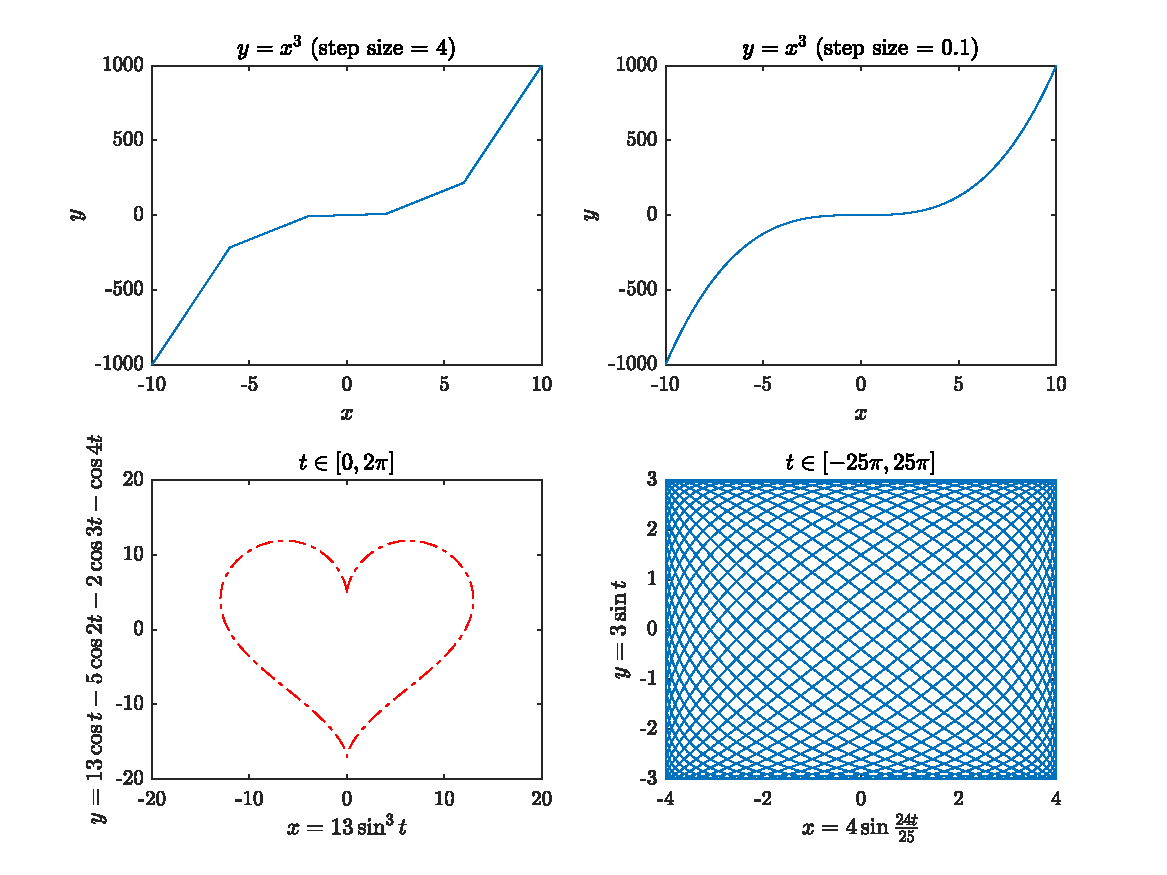
\includegraphics[height=0.27\textheight]{./fig/lab_04_plot_1.pdf}
    \caption{Expected Result for Part 1}
    \label{fig:1}
\end{figure}
\end{enumerate}
%---------------------------------------------
\section{Set Properties for Plotting}
%---------------------------------------------
\begin{enumerate}[(a)]
    \item Define \verb|x|, which ranges from $0$ to $2\pi$ with $1000$ points, and define \verb|y1|, \verb|y2|, and \verb|y3| as follows
        $$
        y_1 = \sin(x/2), \quad
        y_2 = \sin(x), \quad
        y_3 = \sin(2x).
        $$
    \item Plot \verb|y1|, \verb|y2|, \verb|y3| versus \verb|x| in the same figure window with line style (\verb|'LineWidth'|, 2), legend, labels, grid, and title in Figure \ref{fig:2}. Change the range of $x$-axis to $[0, 2\pi]$, and that of $y$-axis to $[-1, 1]$.
\item Use \verb|set| to set the following properties:
    \begin{itemize}
        \item \verb|XTick| to \verb|[0, pi / 2, pi, 3 * pi / 2, 2 * pi]|;
        \item \verb|XTickLabel| to \verb|{'0', '$\pi/2$', '$\pi$', '$3 \pi/2$', '$2\pi$'}|;
        \item \verb|GridLineStyle| to \verb|'--'|;
        \item \verb|Box| to \verb|'on'|;
        \item \verb|BoxStyle| to \verb|'full'|.
    \end{itemize}
\begin{figure}[!hbtp]
    \centering
    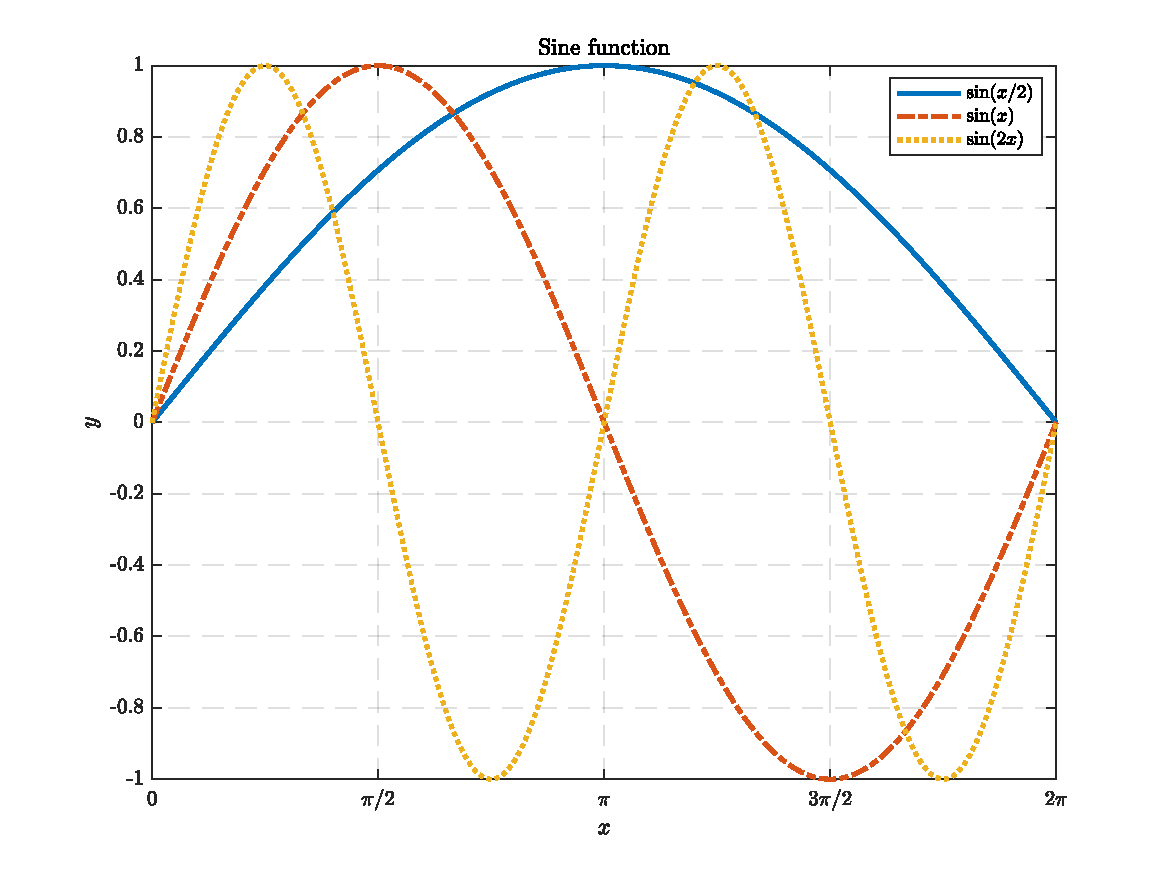
\includegraphics[height=0.27\textheight]{./fig/lab_04_plot_2.pdf}
    \caption{Expected Result for Part 2}
    \label{fig:2}
\end{figure}
\end{enumerate}
%---------------------------------------------
\section{Plotting Piecewise Function on Different Scales}
%---------------------------------------------
\begin{enumerate}[(a)]
    \item Define \verb|x| to be a vector from $0$ to $10$ with step size $0.01$, and the piecewise function \verb|y| as below
        $$
        y =
        \begin{cases}
            \frac{e^{8}}{8} x & x \leq 8, \\
            e^{x} & 8 < x.
        \end{cases}
        $$
    \item \label{enu:3b} In \verb|subplot(2, 2, 1)|, use \verb|plot| to plot \verb|y| versus \verb|x|. Set \verb|grid minor|, add labels and title as shown in the first plot in Figure \ref{fig:3}.
    \item Repeat (\ref{enu:3b}), then set $y$-axis to log scale using \verb|set(gca, 'YScale', 'log');|.
    \item Repeat (\ref{enu:3b}), but use \verb|semilogy| to plot \verb|y| versus \verb|x| instead.
    \item Combine the first and the third figure in \verb|subplot(2, 2, 4)| using \verb|plotyy|, then add labels, title, etc. as shown in the fourth plot in Figure \ref{fig:3}.

\begin{figure}[!hbtp]
    \centering
    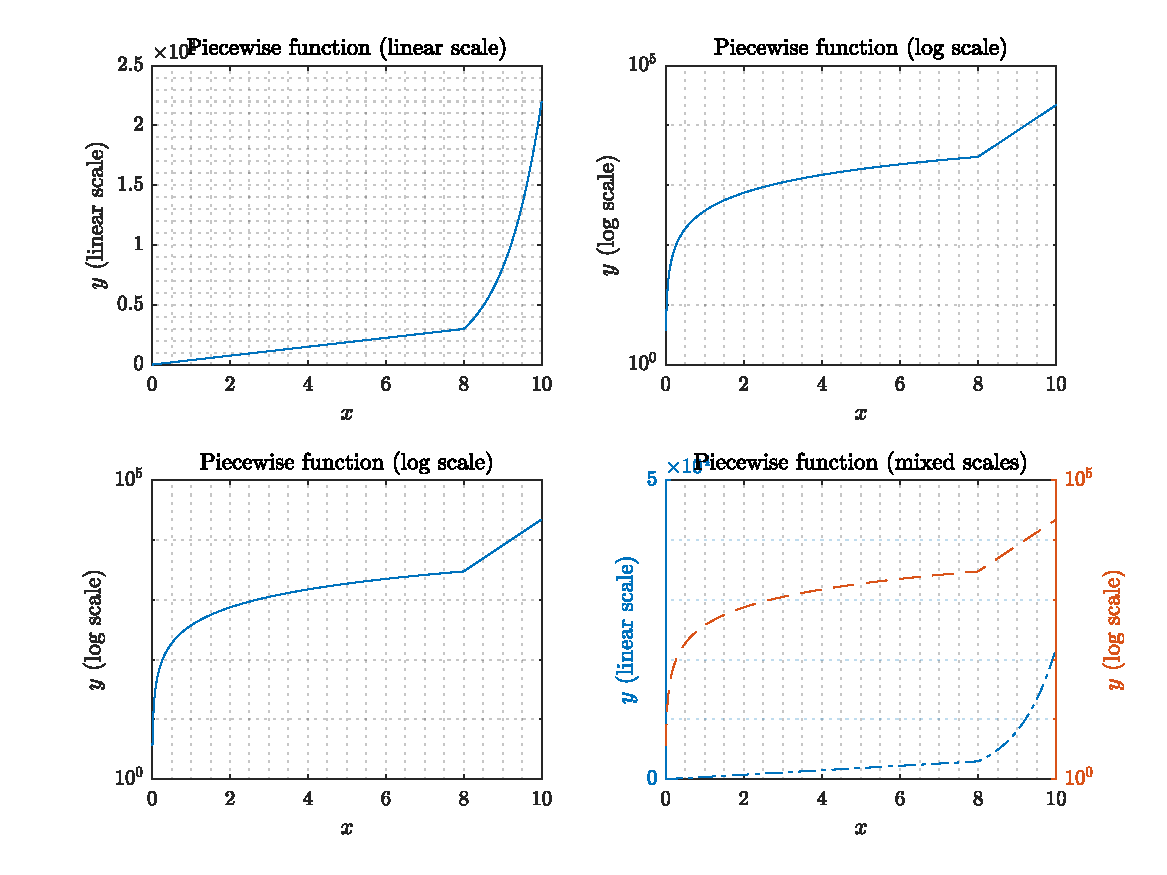
\includegraphics[height=0.25\textheight]{./fig/lab_04_plot_3.pdf}
    \caption{Expected Result for Part 3}
    \label{fig:3}
\end{figure}
\end{enumerate}
%---------------------------------------------
\section{Save Plots}
Use the following script to save the figures.

\begin{lstlisting}[style=MATLAB]
prefix = 'lab_04_plot_';
for i = 1:3
    name = strcat(prefix, num2str(i));       % Set filename for figure i
    fig = figure(i);                         % Set figure i as current figure window
    set(fig, 'PaperPositionMode', 'auto');   % Set paper position mode to 'auto'
    pos = get(fig, 'PaperPosition');         % Get figure window paper position
    set(fig, 'PaperSize', [pos(3) pos(4)]);  % Set figure paper size
    print(fig, '-dpdf', name);               % Save figure
end
\end{lstlisting}

Once you finish, upload the script file \verb|lab_04_script.m| to the folder \verb|src|, figure files \verb|lab_04_plot_1.pdf|,  \verb|lab_04_plot_2.pdf|, and \verb|lab_04_plot_3.pdf| to the folder \verb|figure| on Overleaf. Recompile, and submit the generated \verb|.pdf| file to WyoCourses.
